%!TEX root = ../main.tex

\chapter{Implementation}\label{cha:implementation}

This chapter will explain how the method of fingerprinting was implemented within the Axelrod Python Library.
Each of the definitions presented in Chapter \ref{cha:theory} directly correspond to functions which are described below.
All strategies have an equivalent class within the library and this is demonstrated in Section \ref{sec:fingerprint-implementation}.

\section{The Dual}
The dual of a strategy is defined such that when the original strategy and the dual are presented with identical histories they will return opposite actions, as outlined in Definition \ref{def:dual}.
This means the dual relies on knowledge of how the original strategy would have behaved in a given situation, which is impractical to infer from the source code.
However, the required behaviour can be achieved by having the original strategy as an attribute of the dual.
Whenever the dual has to submit a move, it can first get the original strategy to suggest what move should it would have made, and then flip that action.

\begin{algorithm}[H]
\While{Game is being played}{
  \If{First Turn}{
   create copy of original strategy\;}
  simulate original strategy\;
  update original strategy's history/internal state\;}
  \Return{Flip of original strategy's move}
 \caption{The Dual of a Strategy}
\end{algorithm}

\section{The Joss Ann}

A formal definition of the Joss Ann is given in Section \ref{sec:joss-ann}.
Given a probability distribution $(x, y)$ the Joss Ann Cooperates with probability $x$, Defects with probability $y$, and plays the original move with probability $1 -x-y$.
This can be implemented very simply as seen in Algorithm \ref{alg:joss-ann}.
First, a random number between 0 and 1 is generated.
The thresholds for Cooperation, Defection and original move are then $x, x+y \text{ and } 1$ respectively.

\begin{algorithm}[H]
\While{Game is being played}{
  p $\gets$ Random number\;
  \uIf{p $\leq$ Cooperation Threshold}{
   Next Move $\gets C$\;}
  \uElseIf{p $\leq$ Defection Threshold}{
   Next Move $\gets D$\;}
  \Else{Next Move $\gets$ Original choice of Strategy\;}
  }
  \Return{Next Move}
 \caption{The Joss Ann of a Strategy}
 \label{alg:joss-ann}
\end{algorithm}

\section{Implementation of Fingerprinting}\label{sec:fingerprint-implementation}

As defined in section a fingerprint function is merely the expected score of a strategy when played against a Joss-Ann transformer of a probe with varying parameters (see definition \ref{def:fingerprint}).
As part of this project, a numerical implementation has now been included in the Axelrod-Python library.
It begins by taking a sample of the $x,y$ values that may define the Joss-Ann Transformer.
The strategy then plays a match against a transformer with each of the sampled values.
The average score per turn can be calculated at the end of each match which corresponds to the expected score required by the analytical fingerprint function.
The whole process can be repeated for reliability and the resulting scores plotted.
The player interactions have been modelled as a spatial tournament within Axelrod-Python, where the strategy plays all of the probes and a probe only plays the strategy.
For an example with 9 probes, see Figure \ref{fig:spatialtourn}.

\begin{figure}[!hbtp]
    \begin{center}
        \includestandalone{../img/spatial_tournament}
        \caption{A spatial tournament for the strategy against 9 probes}\label{fig:spatialtourn}
    \end{center}
\end{figure}


Whether the numerical fingerprint matches the analytical one relies heavily on the choice of parameters.
Specifically the \mintinline{python}{turns, repetetitons} and \mintinline{python}{step} variables.
The \mintinline{python}{step} variable determines the number of $x,y$ values taken.
Listing \ref{lst:create-points} shows how a grid of points is constructed over the unit square where the distance between each point is taken as \mintinline{python}{step}.
Therefore, a smaller \mintinline{python}{step} value means more points are created and so greater detail is included in the plot (similar to pixels).

\begin{listing}[hbtp!]
\begin{SourceCode}
def create_points(step):
    """Creates a set of Points over the unit square.
    A Point has coordinates (x, y). This function constructs points that are
    separated by a step equal to `step`. The points are over the unit
    square which implies that the number created will be (1/`step` + 1)^2.
    Parameters
    ----------
    step : float
        The separation between each Point. Smaller steps will produce more
        Points with coordinates that will be closer together.
    Returns
    ----------
    points : list
        of Point objects with coordinates (x, y)
    """
    num = int((1 / step) // 1) + 1
    points = [Point(j, k) for j in np.linspace(0, 1, num)
              for k in np.linspace(0, 1, num)]

    return points
\end{SourceCode}
\caption{Axelrod-Python code to create a sample of $x,y$ points}
\label{lst:create-points}
\end{listing}

The \mintinline{python}{turns} variable determines how many interactions there will be in a match.
Enough turns must be selected to ensure that steady long term behaviour is reached otherwise the average score per turn can be wildly innacurate.
However, once this state is reached, extending the number of turns has a minimal effect on the accuracy of the plot.
The \mintinline{python}{repetitions} variable decides how many times the tournament would be repeated.
The Axelrod-Python implementation of fingerprinting is a random process (due to the Joss-Ann) and high repetitions helps to reduce the effects of this.


\section{Comparison of Analytical and Numerical Plots}

In figure \ref{fig:ashlock-fingerprints}, several analytical fingerprints from previous literature are shown \cite{Ashlock2004, Ashlock2008}.
Colourings or shadings are used to make certain features stand out, and an attempt to replicate this behaviour was implemented in Axelrod-Python.
The popular plotting library, matplotlib, has many options for different colour maps which are demonstrated in Appendix . %TODO - appendix reference

\begin{figure}[hbtp!]
    \begin{center}
        \includegraphics[width = 0.6\textwidth]{../img/MultipleFingerprintsAshlock}
    \end{center}
    \caption{Shaded plots of the fingerprint functions for the strategies TitForTat, Psycho, AllD and AllC, in reading order from \cite{Ashlock2004}}
    \label{fig:ashlock-fingerprints}
\end{figure}

Using the analytical fingerprints from previous literature \cite{Ashlock2004, Ashlock2008}, and the fingerprint formulae provided alongside them, the most appropriate colour map was chosen.
The colour map Seismic \cite{matplotlib-colormap} was selected due to its divergent properties (although all colour maps are available within the library).
With divergent colour maps, all extreme values (high or low) are coloured, whilst mid range values are left white \cite{Moreland2009}.
This highlights areas of interest, and in Figure \ref{fig:WSLS-ashlock-comparison} it can be seen that this matches previous work well.

\begin{figure}[hbtp!]
\centering
\subfloat[WSLS fingerprint from previous literature \cite{Ashlock2008}]{
\includegraphics[width = 0.4\textwidth]{../img/WSLS-Ashlock}}
\subfloat[Analytical WSLS fingerprint demonstrating Seismic colouring]{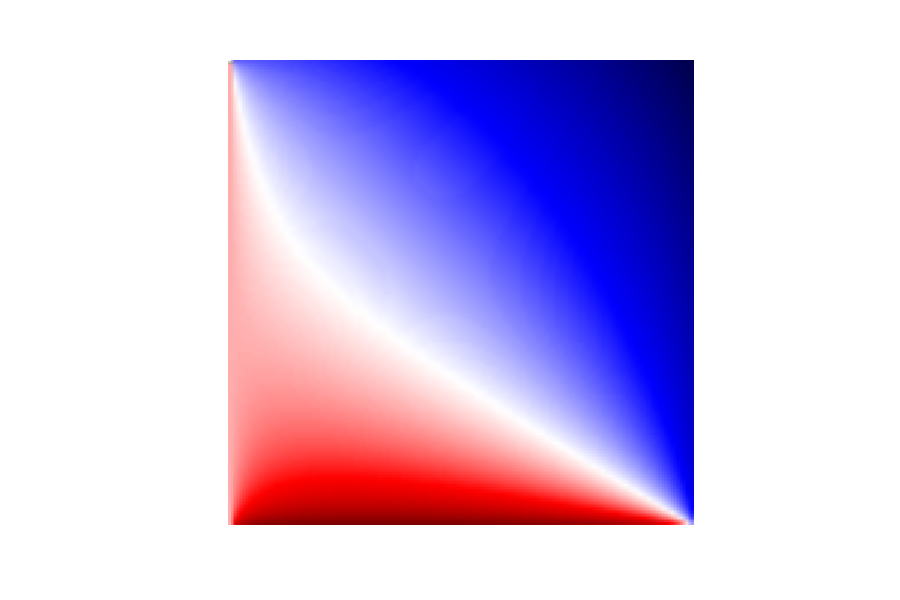
\includegraphics[width = 0.7\textwidth]{../img/WSLS-Analytical}}
\caption{A comparison of a fingerprint plot from previous literature to asses the suitability of the Seismic colour map \cite{Ashlock2008}}
\label{fig:WSLS-ashlock-comparison}
\end{figure}

With the knowledge that the choice of colourmap is appropriate, a comparison can now be made between analytical fingerprints and numerical ones obtained via the Axelrod-Python library.
Table \ref{tab:fingerprint-functions} gives the analytical fingerprint functions of several well known strategies that will then be used to validate the numerical versions.

\begin{table}[htbp!]
\centering
\renewcommand{\arraystretch}{2}
\setlength{\tabcolsep}{12pt}
\begin{tabular}{l l}
\toprule
Strategy & Analytical Fingerprint Function\\
\midrule
TitForTat &  $\displaystyle \frac{y^2 + 5xy + 3x^2}{(x + y)^2} $\\
Psycho (Anti TitForTat& $\displaystyle \frac{4(y-1)(x-1) + 5(y-1)^2}{2(y-1)(x-1) + (x-1)^2 + (y-1)^2} $ \\
WinStayLoseShit (Pavlov) & $\displaystyle \frac{(3x+y)(x-1) + 5y(y-1)}{(x+2y)(x-1) + y(y-1)} $\\
AllC (Cooperator) & $\displaystyle 3 - 3y $ \\
AllD (Defector) & $\displaystyle 4x + 1 $\\
\bottomrule
\end{tabular}
\caption{A selection of analytical fingerprint functions for well known strategies. The probe used is TitForTat.}
\label{tab:fingerprint-functions}
\end{table}

Figures \ref{fig:TFT-comparison} \ref{fig:Psycho-comparison} \ref{fig:WSLS-comparison} \ref{fig:Cooperator-comparison} \ref{fig:Defector-comparison} compare plots of known analytical fingerprint functions with numerical approximations obtained with the Axelrod-Python library.
The analytical plots were created with the code seen in listing \ref{lst:create-several-fingerprints}.
The parameters \mintinline{python}{turns=500, repetitions=200, step=0.01} are as described in section \ref{sec:fingerprint-implementation}.
The parameter \mintinline{python}{processes=0} ensures that the function will use the maximum number of cores available on the computer.

\begin{listing}[hbtp!]
\begin{ExampleCode}
import axelrod as axl
strats = [axl.TitForTat, axl.WinStayLoseShift, axl.AntiTitForTat,
          axl.Cooperator, axl.Defector]
for s in strats:
    probe = axl.TitForTat
    af = axl.AshlockFingerprint(s, probe)
    data = af.fingerprint(turns=500, repetitions=200, step=0.01, processes=0)
    p = af.plot()
    p.savefig('{}-Numerical.pdf'.format(s.name))
\end{ExampleCode}
\caption{Code to create the numerical plots for several strategies}
\label{lst:create-several-fingerprints}
\end{listing}

\begin{figure}[htbp!]
\subfloat[Exact analytical fingerprint]{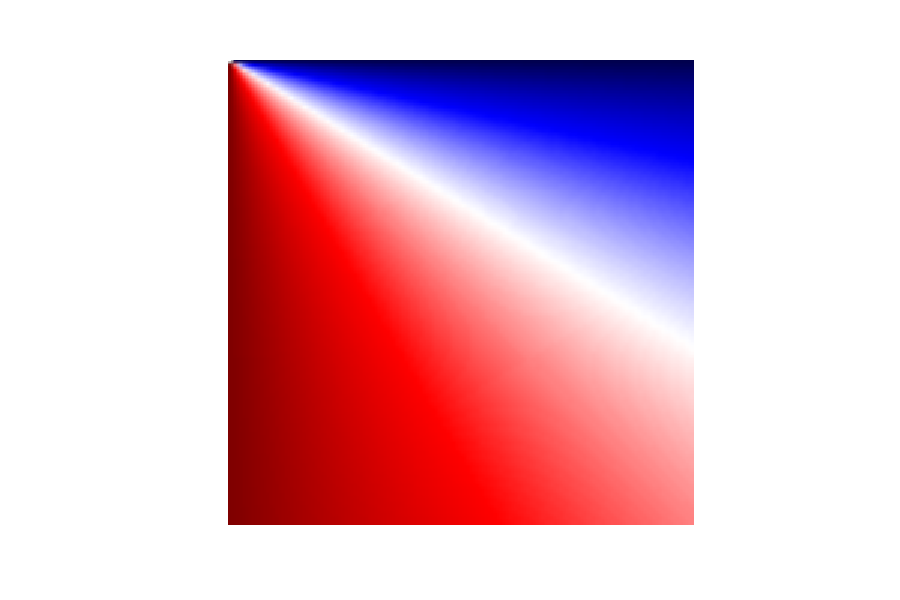
\includegraphics[width = 0.5\textwidth]{../img/TFT-Analytical.pdf}}
\subfloat[Numerical Fingerprint]{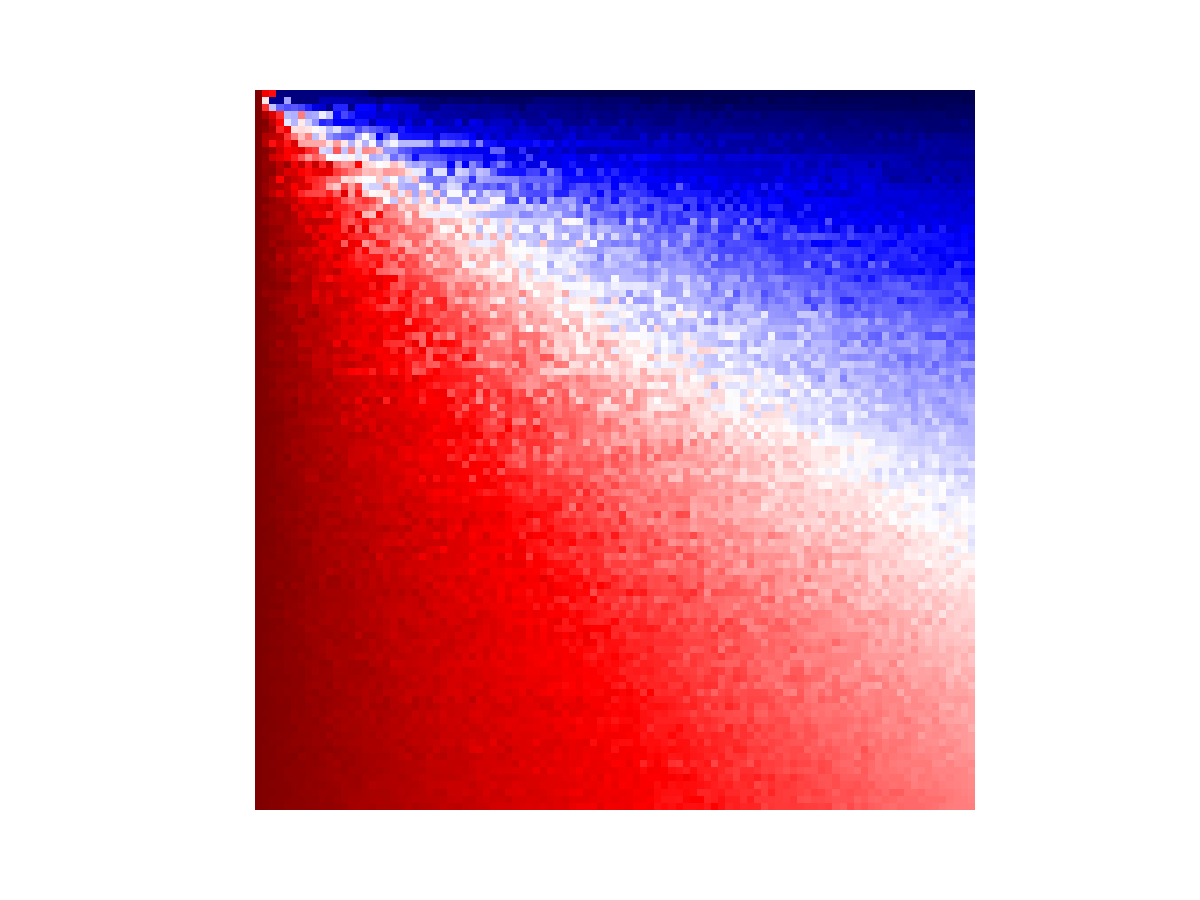
\includegraphics[width = 0.5\textwidth]{../img/Numerical/TitForTat.pdf}}
\caption{A comparison of the analytical fingerprint of TitForTat and the numerical version produced by Axelrod-Python library.}
\label{fig:TFT-comparison}
\end{figure}
\begin{figure}[htbp!]
\subfloat[Exact analytical fingerprint]{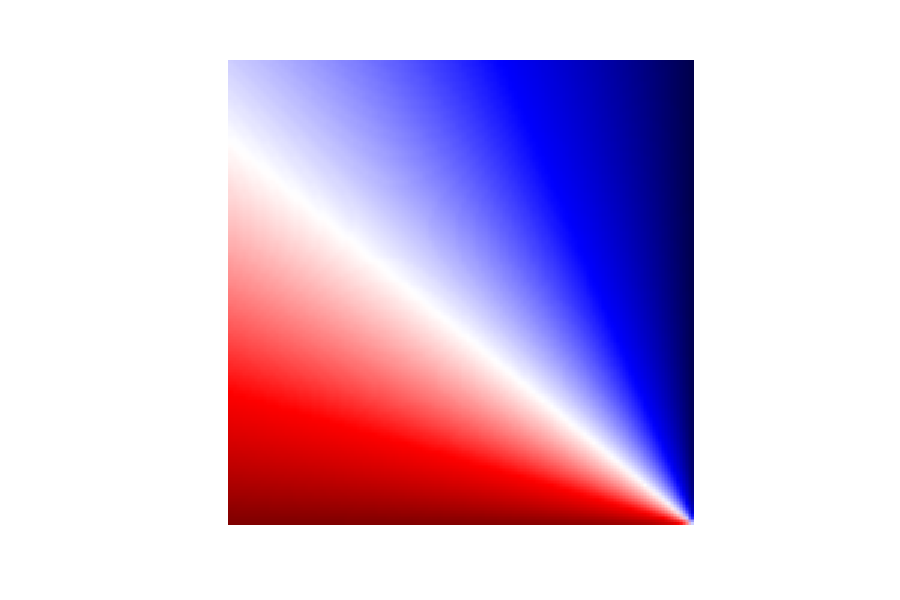
\includegraphics[width = 0.5\textwidth]{../img/Psycho-Analytical.pdf}}
\subfloat[Numerical Fingerprint]{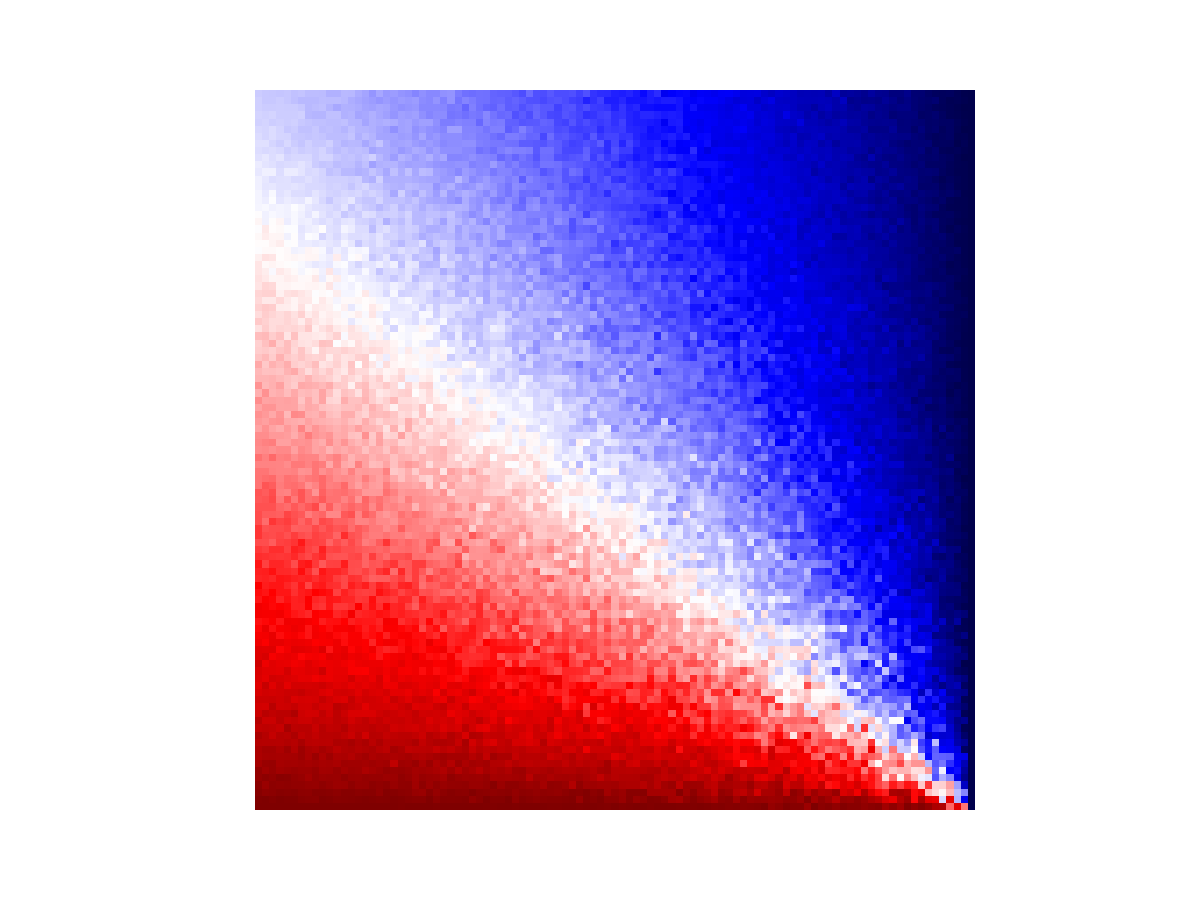
\includegraphics[width = 0.5\textwidth]{../img/Numerical/AntiTitForTat.pdf}}
\caption{A comparison of the analytical fingerprint of Psycho and the numerical version produced by Axelrod-Python library.}
\label{fig:Psycho-comparison}
\end{figure}
\begin{figure}[htbp!]
\subfloat[Exact analytical fingerprint]{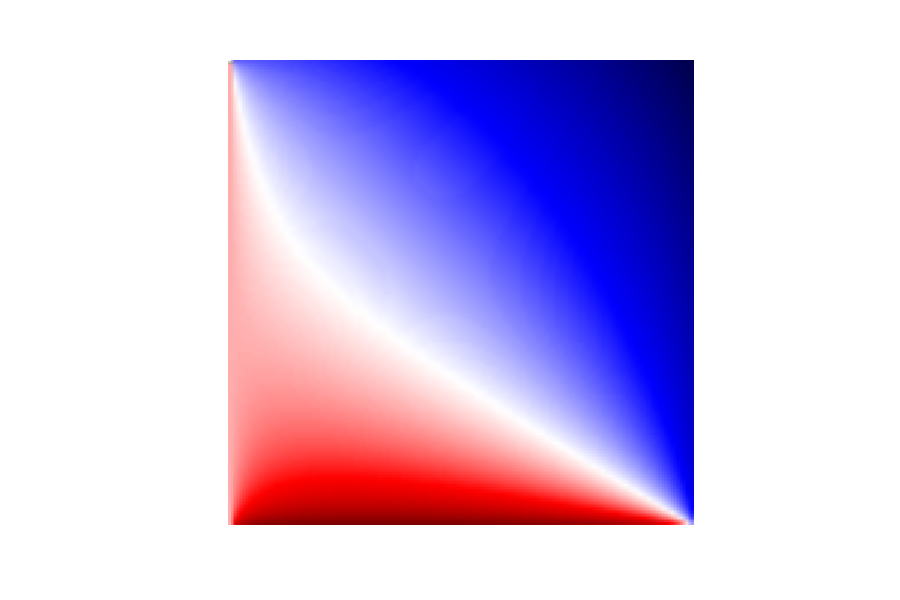
\includegraphics[width = 0.5\textwidth]{../img/WSLS-Analytical.pdf}}
\subfloat[Numerical Fingerprint]{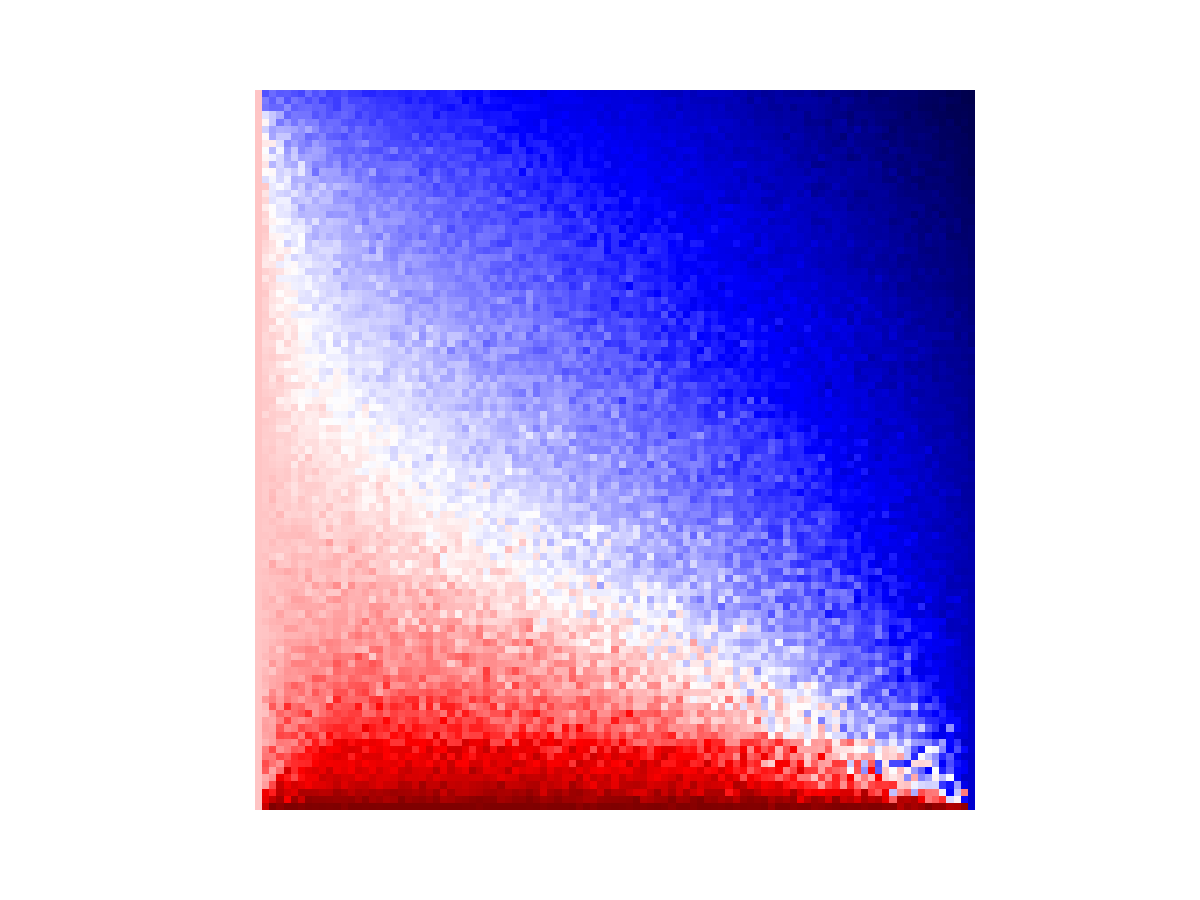
\includegraphics[width = 0.5\textwidth]{../img/Numerical/Win-Stay-Lose-Shift.pdf}}
\caption{A comparison of the analytical fingerprint of WinStayLoseShit and the numerical version produced by Axelrod-Python library.}
\label{fig:WSLS-comparison}
\end{figure}
\begin{figure}[htbp!]
\subfloat[Exact analytical fingerprint]{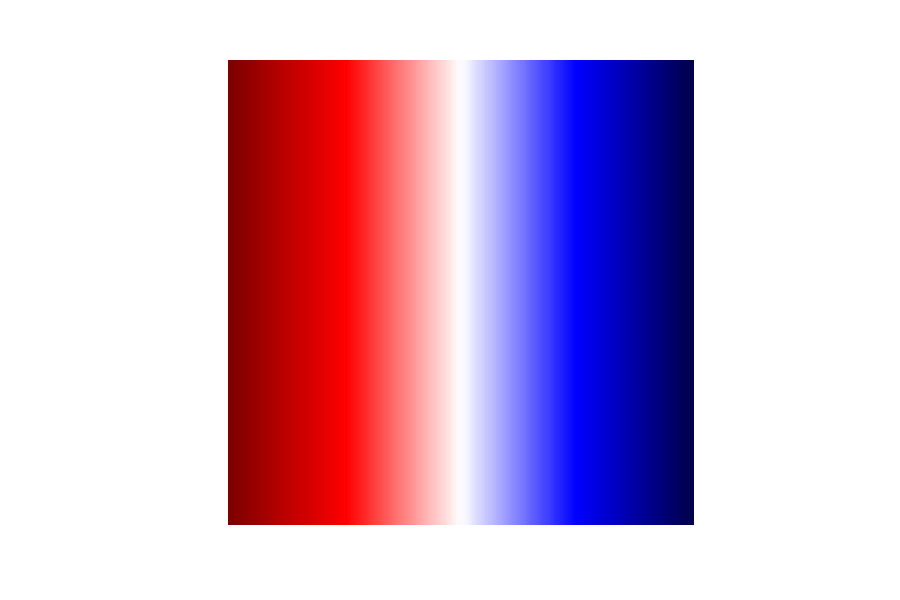
\includegraphics[width = 0.5\textwidth]{../img/AllC-Analytical.pdf}}
\subfloat[Numerical Fingerprint]{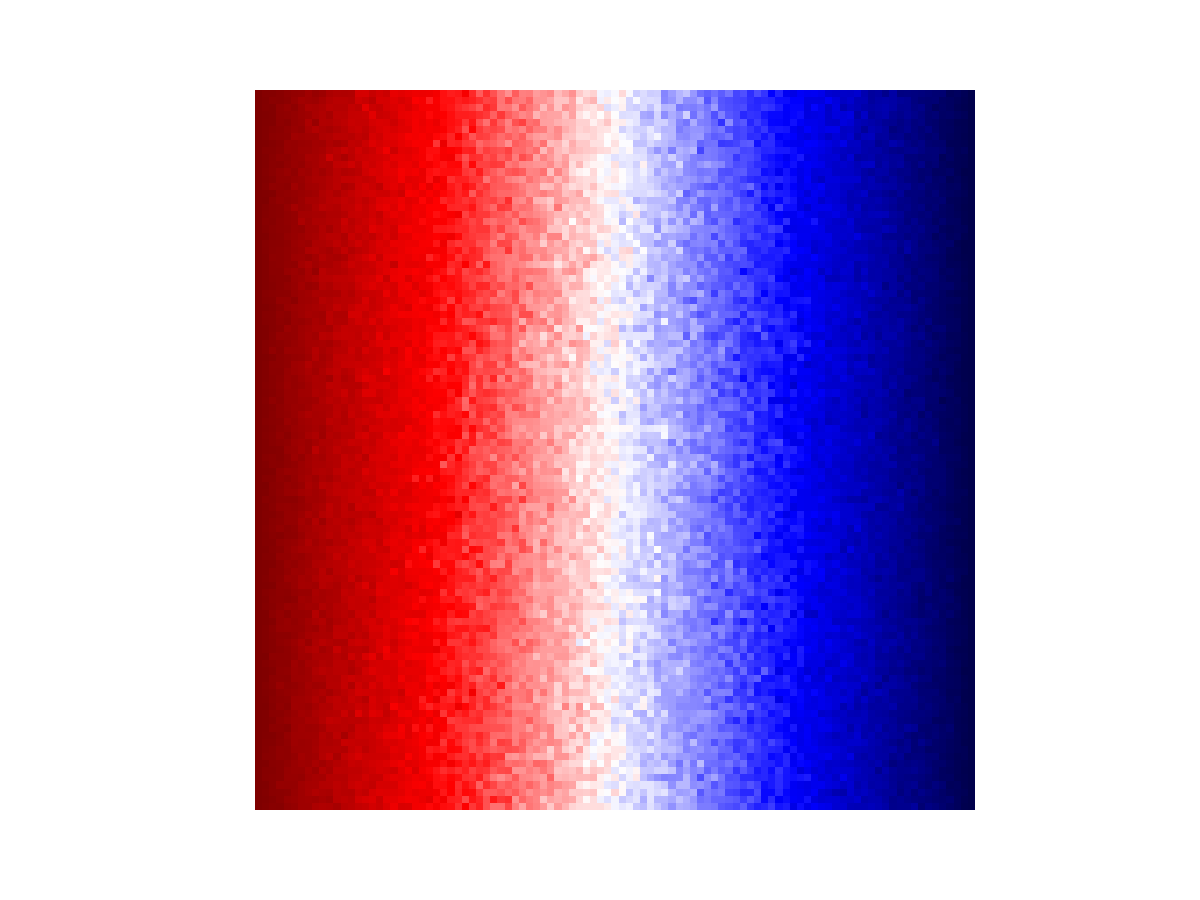
\includegraphics[width = 0.5\textwidth]{../img/Numerical/Cooperator.pdf}}
\caption{A comparison of the analytical fingerprint of Cooperator and the numerical version produced by Axelrod-Python library.}
\label{fig:Cooperator-comparison}
\end{figure}
\begin{figure}[htbp!]
\subfloat[Exact analytical fingerprint]{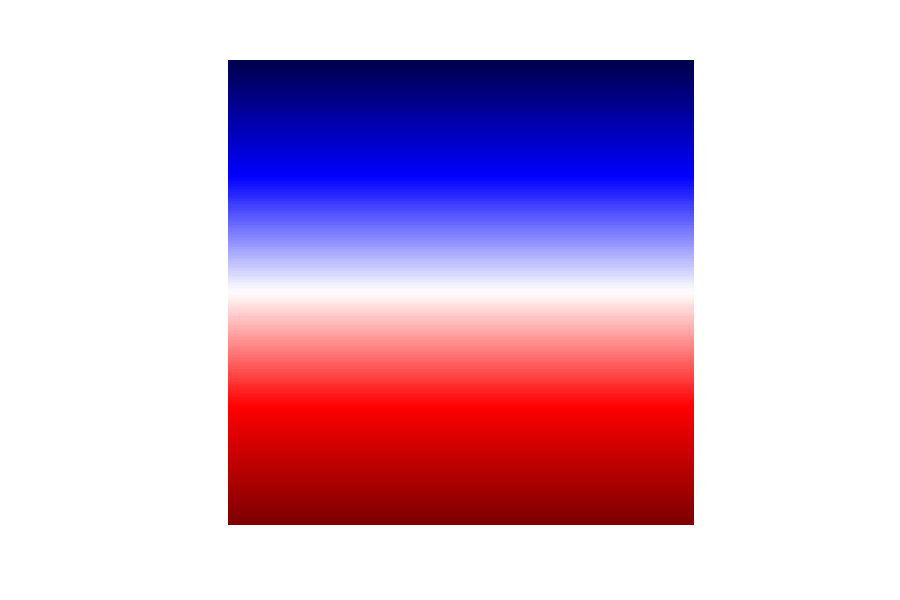
\includegraphics[width = 0.5\textwidth]{../img/AllD-Analytical.pdf}}
\subfloat[Numerical Fingerprint]{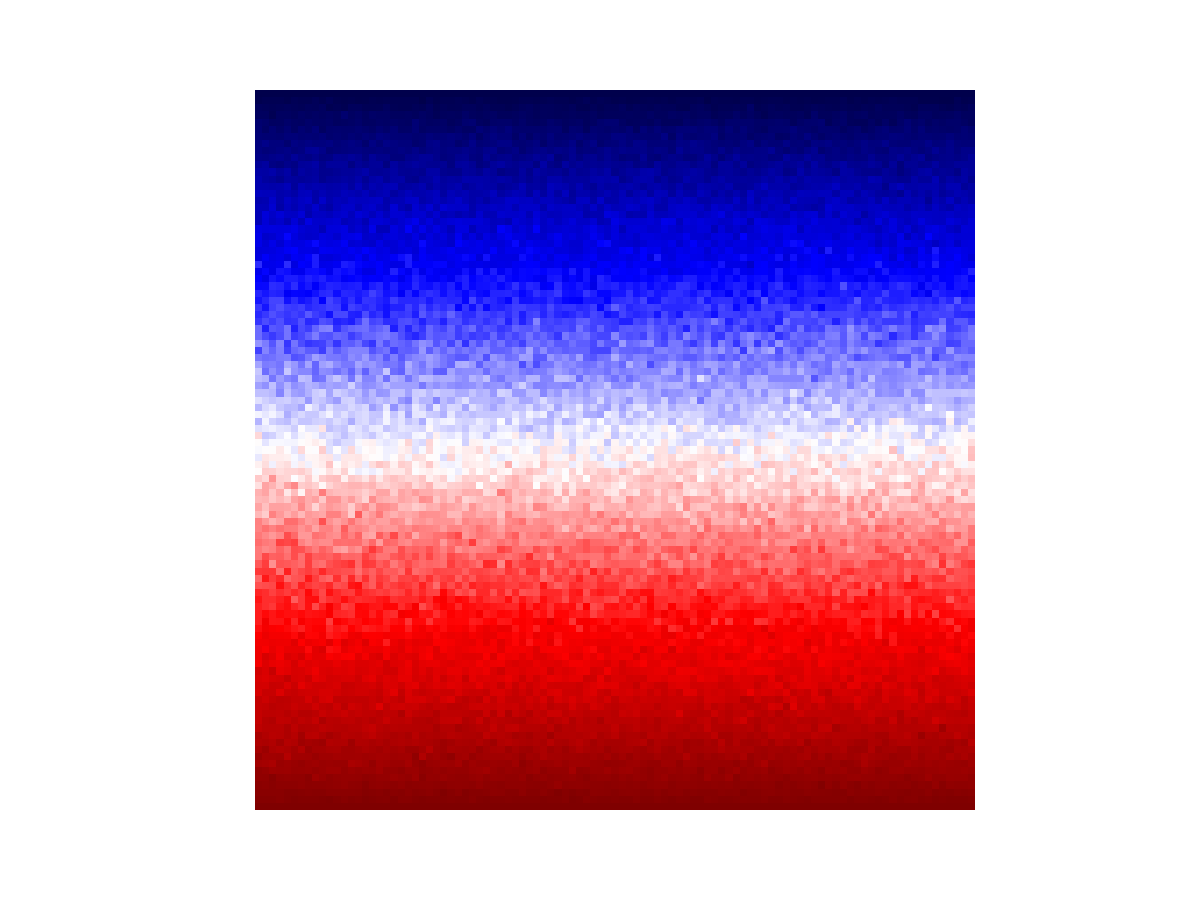
\includegraphics[width = 0.5\textwidth]{../img/Numerical/Defector.pdf}}
\caption{A comparison of the analytical fingerprint of Defector and the numerical version produced by Axelrod-Python library.}
\label{fig:Defector-comparison}
\end{figure}

\section{The Development Process}\label{sec:dev_process}

The Axelrod-Python library aims to follow best practice at all times with regards to development.
The source code is hosted at Github and all code is version controlled.
Version control ensures that all changes to a code base are tracked and can be traced back to a particular author.
It also allow different developers to make sure that they are using the same version of the software, particularly important with regards to reproducing results.

The library also applies a strict review process, where any code submission is analysed by several members of the organisation before it can be included.
This normally involves other developers requesting changes to the submission, this ensure that all source code is of the same high standard.
Figure \ref{fig:screenshots} shows some screen shots of the discussions, requests and suggestions made during the development process of the fingerprint code.

\begin{figure}[htbp!]
\ContinuedFloat
\centering
\subfloat[Exact analytical fingerprint]{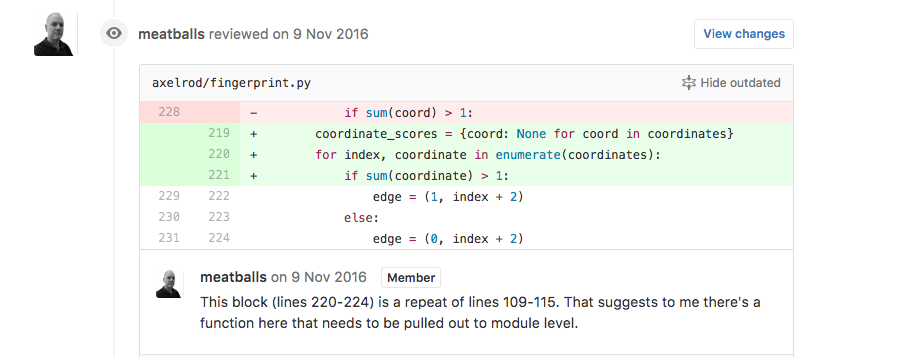
\includegraphics[width = \textwidth]{../img/screenshots/ScreenShot1.png}}

\ContinuedFloat
\subfloat[Exact analytical fingerprint]{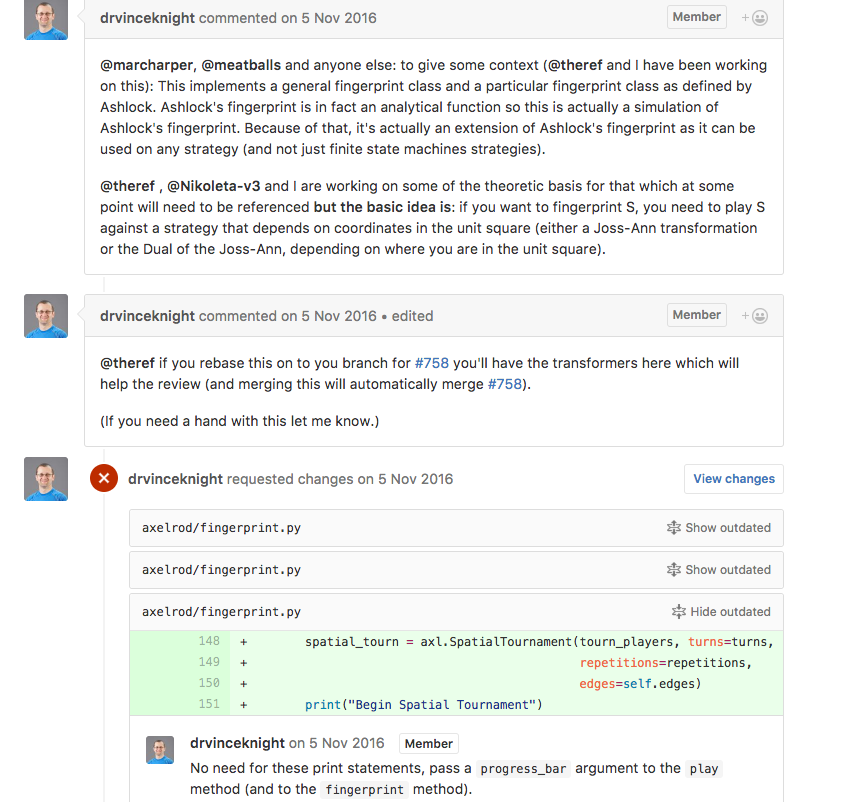
\includegraphics[width = \textwidth]{../img/screenshots/ScreenShot2.png}}

\ContinuedFloat
\subfloat[Exact analytical fingerprint]{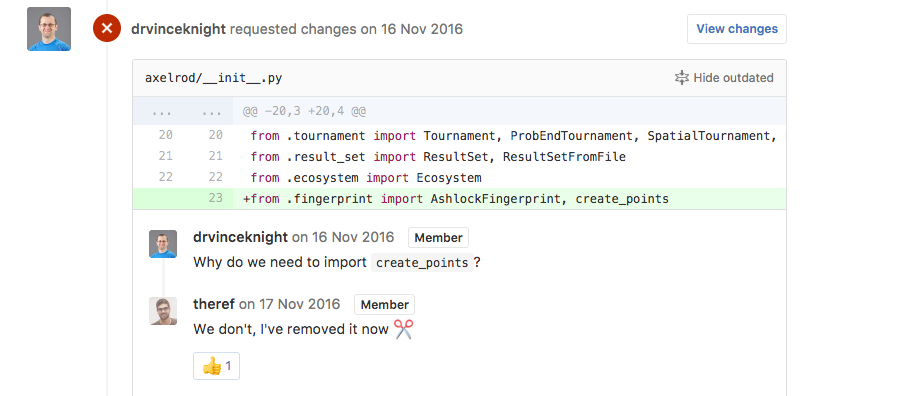
\includegraphics[width = \textwidth]{../img/screenshots/ScreenShot3.png}}

\ContinuedFloat
\subfloat[Exact analytical fingerprint]{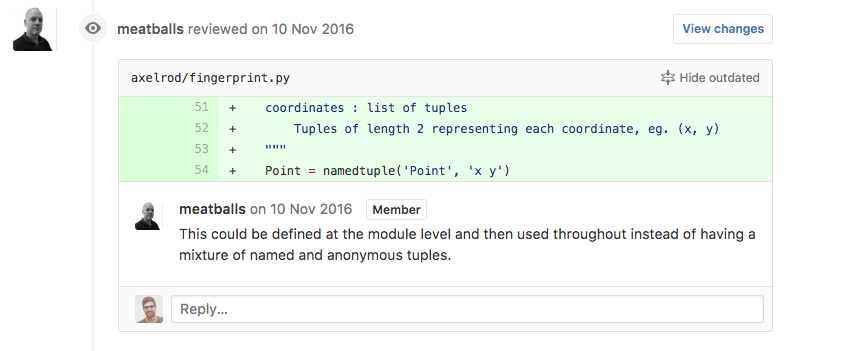
\includegraphics[width = \textwidth]{../img/screenshots/ScreenShot4.png}}

\caption{Screen shots of the discussion for fingerprint code submission.}
\label{fig:screenshots}
\end{figure}
% \section{Axelrod Python}

% The Axelrod-Python library is equipped with an extensive tests suite and all code is comprehensively documented.
% The documentation can be found at \url{http://axelrod.readthedocs.io/en/latest/} along with several tutorials designed to help introduce researchers to the library.
% In total the library now consists of 147 strategies (at the time of writing) including classical ones from the literature and and some exciting original contributions.
% It is interesting that the original winner, TitForTat, is currently ranked 49th overall.
% The library also has the capability to run ecological simulations or construct tournaments on alternative topologies (not just the original round robin format).

% An example implementation of a strategy and a demonstration of using the library will now be given, followed by examples of some of the many plots the library can produce.
% The source code for TitForTat is shown in Listing \ref{lst:TFT}.

% \begin{listing}[htbp!]
% \begin{SourceCode}
% class TitForTat(Player):
%     """
%     A player starts by cooperating and then mimics the previous action of the
%     opponent.

%     Note that the code for this strategy is written in a fairly verbose
%     way. This is done so that it can serve as an example strategy for
%     those who might be new to Python.

%     Names:

%     - Rapoport's strategy: [Axelrod1980]_
%     - TitForTat: [Axelrod1980]_
%     """

%     # These are various properties for the strategy
%     name = 'Tit For Tat'
%     classifier = {
%         'memory_depth': 1,  # Four-Vector = (1.,0.,1.,0.)
%         'stochastic': False,
%         'makes_use_of': set(),
%         'long_run_time': False,
%         'inspects_source': False,
%         'manipulates_source': False,
%         'manipulates_state': False
%     }

%     def strategy(self, opponent):
%         """This is the actual strategy"""
%         # First move
%         if not self.history:
%             return C
%         # React to the opponent's last move
%         if opponent.history[-1] == D:
%             return D
%         return C
% \end{SourceCode}
% \caption{Source code for TitForTat}
% \label{lst:TFT}
% \end{listing}

% Strategies are implemented as classes with a \mintinline{python}{strategy} method.
% The strategy method contains the logic that defines how the strategy will behave as can be seen in listing \ref{lst:TFT} lines 28 - 36.
% If the player does not have a history then it must be the first move and it chooses to play `C'.
% On all subsequent moves the player checks whether the opponent played `D' on it's previous move.
% If that statement is true the player also plays `D', otherwise it will play `C'.
